% Artigo para Cadernos de Saúde Pública (CSP), categoria Artigo: até 6.000 palavras (corpo + referências) e 5 ilustrações.
%
% Este projeto é a pasta artigo/latex/ do repositório; é o que sobe no Overleaf.
%   - tabelas/*.tex e figuras/*.pdf são gerados pela análise (artigo/analise/para_latex.py): não edite à mão.
%   - Os números do texto estão digitados e foram conferidos com artigo/resultados/numeros.json (rodada de 19/11/2026).
%   - Comentários: \thiago{...}, \vini{...}, \victor{...}; trechos a escrever: \pendente{...}.
% Na submissão, a CSP pede texto, tabelas, figuras e legendas em arquivos separados (DOC/DOCX): isso se faz no fim.

\documentclass[12pt,a4paper]{article}

\usepackage[T1]{fontenc}
\usepackage[utf8]{inputenc}
\usepackage[brazilian]{babel}
\usepackage{newtxtext}                  % Times
\usepackage[margin=2cm]{geometry}       % margens de 2 cm
\usepackage{setspace}\onehalfspacing    % entrelinha 1,5
\usepackage{amsmath,amssymb,amsthm}     % usados por macros.tex
\usepackage{xcolor}
\usepackage{graphicx}
\usepackage{booktabs}
\usepackage{array}
\usepackage{float}
\usepackage[font=small,labelfont=bf,labelsep=period]{caption}
\captionsetup[table]{position=top}
\usepackage[super,sort&compress]{natbib} % referências numeradas em sobrescrito
\usepackage{xurl}
\usepackage[hidelinks]{hyperref}

% coluna alinhada à direita com quebra de linha (usada nas tabelas)
\newcolumntype{R}[1]{>{\raggedleft\arraybackslash}p{#1}}
\DeclareUnicodeCharacter{2212}{\textminus}  % sinal de menos (−) colado de outros arquivos
\setcounter{secnumdepth}{0}                 % seções sem número, como na CSP

% Macros e ambientes compartilhados. Carregar apos os pacotes no main.tex.

% Ambientes e numeracao
\newcounter{dummy}
\numberwithin{dummy}{section}
\newtheorem{theorem}[dummy]{Theorem}
\newtheorem{proposition}[dummy]{Proposition}
\newtheorem{corollary}[dummy]{Corollary}
\newtheorem{lemma}[dummy]{Lemma}
\newtheorem{question}[dummy]{Question}
\newtheorem{conjecture}[dummy]{Conjecture}
\newenvironment{claim}[1]{\par\noindent\underline{Afirma\c{c}\~ao:}\space#1}{}
\newenvironment{claimproof}[1]{\par\noindent\underline{Prova da afirma\c{c}\~ao:}\space#1}{\hfill $\blacksquare$}

\theoremstyle{definition}
\newtheorem{definition}[dummy]{Definition}
\newtheorem{example}[dummy]{Example}
\newtheorem{xca}[dummy]{Exercise}

\theoremstyle{remark}
\newtheorem{remark}[dummy]{Remark}

\numberwithin{equation}{section}

% Conjuntos e categorias
\newcommand{\C}{{\mathbb C}}
\newcommand{\R}{{\mathbb R}}
\newcommand{\N}{\mathbb N}
\newcommand{\Z}{\mathbb Z}
\newcommand{\Q}{{\mathbb{Q}}}
\newcommand{\T}{\mathbb{T}}
\newcommand{\catname}[1]{{\normalfont\textbf{#1}}}
\newcommand{\Set}{\catname{Set}}
\newcommand{\Top}{\catname{Top}}
\newcommand{\Rel}{\catname{Rel}}

% Notacao caligrafica
\newcommand{\X}{\mathcal{X}}
\newcommand{\Y}{\mathcal{Y}}
\newcommand{\A}{\mathcal{A}}
\newcommand{\F}{\mathcal{F}}
\renewcommand{\L}{\mathcal{L}}
\newcommand{\cH}{\mathcal{H}}
\newcommand{\W}{\mathcal{W}}
\newcommand{\Sss}{{\mathcal{S}}}
\newcommand{\LL}{{\mathcal{L}}}
\newcommand{\LLl}{\mathbb{L}}
\newcommand{\QQ}{{\mathcal{Q}}}
\newcommand{\Aa}{{\mathcal{A}}}
\newcommand{\VV}{{\mathcal{V}}}
\newcommand{\BB}{\mathcal{B}}
\newcommand{\MMM}{{\mathcal{M}}}
\newcommand{\CO}{{\mathcal{O}}}
\newcommand{\CW}{{\mathcal{W}}}
\newcommand{\CB}{{\mathcal{B}}}
\newcommand{\CH}{{\mathcal{H}}}
\newcommand{\Ol}{\mathcal{O}}

% Outros simbolos e alfabetos
\newcommand{\Ss}{{\mathfrak{S}}}
\newcommand{\BBB}{{\mathfrak{B}}}
\newcommand{\TTT}{{\mathfrak{T}}}
\newcommand{\Lab}{\underline{\Lambda}}
\newcommand{\PP}{{\mathsf{P}}}
\newcommand{\HH}{{\mathrm{H}}}
\newcommand{\KK}{{\mathrm{K}}}
\newcommand{\Gg}{{\mathsf{G}}}
\newcommand{\Ff}{{\mathsf{F}}}
\newcommand{\EE}{{\mathrm{E}}}
\newcommand{\MM}{{\mathrm{M}}}
\newcommand{\XX}{{\mathrm{X}}}
\newcommand{\ZZ}{{\mathrm{Z}}}
\newcommand{\MMs}{\small{\MM}}
\newcommand{\III}{{\mathfrak{I}}}
\newcommand{\ff}{\mathfrak{F}}
\newcommand{\RR}{\mathrm{R}}
\newcommand{\TT}{{\mathrm{T}}}
\newcommand{\NN}{{\mathfrak{N}}_0}
\newcommand{\DD}{\mbox{D}}
\newcommand{\Kk}{\mathsf{K}}
\newcommand{\OO}{{\mathrm{O}}}
\newcommand{\Sol}{{\mathfrak{S}}}
\newcommand{\mm}{{\mathsf{m}}}
\newcommand{\ha}{\small{\mathrm{ha}}}

% Calculo e analise
\newcommand{\dd}{{\mathrm{d}}}
\newcommand{\ddt}{\partial_t}
\newcommand{\ddxk}{\frac{\partial}{\partial x_k}}
\newcommand{\Ci}{{\mathcal{C}}^\infty}
\newcommand{\Cci}{{\mathcal{C}}^\infty}
\newcommand{\Dli}{{\mathcal{D}}'}
\newcommand{\Eli}{{\mathcal{E}}'}
\newcommand{\sql}{{\ell^{1/2}}}
\newcommand{\ssql}{{\ell^{1/4}}}
\newcommand{\cl}{\mathrm{Cl}\,}
\newcommand{\bmo}{\small \mathrm{bmo}}
\newcommand{\loc}{\small \mathrm{loc}}
\newcommand{\sxi}{\sqrt{\xi}}
\newcommand{\dbar}{\overline{\partial}}
\newcommand{\sS}{\subset\!\!\subset}
\newcommand{\eeps}{\widehat{\otimes}}
\newcommand{\Ome}{{\Omega^\eps}}
\newcommand{\trb}{|||}
\newcommand{\til}{\widetilde}
\newcommand{\brr}{\overline}
\newcommand{\iprod}{\mathbin{\lrcorner}}
\newcommand{\TP}{\ ^t P}
\newcommand{\TK}{\ ^t K}
\newcommand{\Tt}{\ ^tT}
\newcommand{\tr}[1]{\mathrm{tr}\left\{#1\right\}}

% Operadores
\newcommand{\sgn}{\mbox{sgn}}
\newcommand{\Div}{\mbox{div}}
\DeclareMathOperator{\GL}{GL}
\DeclareMathOperator{\spn}{span}
\DeclareMathOperator{\pr}{pr}
\DeclareMathOperator{\Aut}{Aut}
\DeclareMathOperator{\ran}{ran}
\DeclareMathOperator{\aut}{aut}
\DeclareMathOperator{\Hol}{Hol}
\DeclareMathOperator{\hol}{hol}
\DeclareMathOperator{\supp}{supp}
\DeclareMathOperator{\intr}{int}
\DeclareMathOperator{\Jac}{Jac}
\DeclareMathOperator{\ddleb}{\dd \mathrm{m}}
\DeclareMathOperator{\RE}{Re}
\DeclareMathOperator{\IM}{Im}
\DeclareMathOperator{\vol}{vol}
\DeclareMathOperator{\RI}{RI}
\DeclareMathOperator{\dvol}{dvol}

% Probabilidade
\newcommand{\Ind}[1]{\mathbb{I}\left\lbrace#1\right\rbrace}
\newcommand{\Var}[1]{\mathrm{Var}\left[#1\right]}
\newcommand{\Varx}[2]{\mathrm{Var}_{#1}\left[#2\right]}
\newcommand{\Cov}[1]{\mathrm{Cov}\left(#1\right)}
\newcommand{\E}[1]{\mathbb{E}\left[#1\right]}
\newcommand{\Ex}[2]{\mathbb{E}_{#1}\left[#2\right]}
\renewcommand{\Pr}[1]{\mathbb{P}\left(#1\right)}
\newcommand{\Prx}[2]{\mathbb{P}_{#1}\left(#2\right)}



\newcommand{\thiago}[1]{{\color{red} Thiago:  #1}}
\newcommand{\vini}[1]{{\color{blue} Vini:  #1}}

\newcommand{\victor}[1]{{\color{teal} Victor:  #1}}
\newcommand{\pendente}[1]{{\color{orange}[#1]}}

\title{Bets e saúde mental no Brasil: jogo patológico no SUS, 2018--2026}
\author{}
\date{}

\begin{document}

\maketitle

% ---------------------------------------------------------------------------------------------------------------------
\section*{Resumo}

\pendente{RASCUNHO, a revisar com os coautores depois da Introdução e da Discussão.} A expansão das apostas de quota fixa no Brasil a partir de 2018 levantou preocupação com o jogo patológico, mas há pouca informação sobre sua repercussão nos serviços de saúde. Este estudo descreve os registros de jogo patológico (CID-10 F63.0) na atenção primária à saúde (APS) e nos Centros de Atenção Psicossocial (CAPS) do Sistema Único de Saúde entre 2018 e 2026, com dados públicos agregados. Os registros de jogo foram expressos por 10 mil registros de depressão, ansiedade, estresse, uso de álcool e esquizofrenia, e outros transtornos dos impulsos (F63.1--F63.3) serviram de controle negativo. A tendência mensal foi analisada por regressão segmentada (\emph{joinpoint}). De 2018 a 2025, os registros de jogo passaram de 95 para 3.423 na APS e de 335 para 4.371 nos CAPS. Na APS, a taxa de jogo passou a crescer 100\% ao ano (IC95\%: 91; 110) a partir de jun/2022; nos CAPS, 181\% ao ano (IC95\%: 107; 367) a partir de mai/2024. O controle negativo pouco variou. Os registros se concentraram entre 25 e 44 anos, e os atendimentos por jogo na APS terminaram menos em alta e foram mais encaminhados a serviço especializado do que os de outros diagnósticos. O registro de jogo patológico no SUS cresceu muito além da demanda de saúde mental e de transtornos com a mesma codificação, começando pela APS. Os dados descrevem atendimentos, e não prevalência, e não permitem separar aumento de casos de aumento do reconhecimento do problema.

\noindent\textbf{Palavras-chave:} Jogo de Azar; Saúde Mental; Atenção Primária à Saúde; Serviços de Saúde Mental

% ---------------------------------------------------------------------------------------------------------------------
\section{Introdução}

\pendente{A ESCREVER: história e cronologia das apostas no Brasil (Lei nº 13.756/2018, Lei nº 14.790/2023, mercado regulado desde janeiro de 2025, CPI das Bets, MP nº 1.394/2026); organização da rede de saúde mental (atenção primária e CAPS); objetivo.}

\pendente{Sugestão para o último parágrafo, alinhada aos métodos: Este estudo descreve a evolução dos registros de jogo patológico na atenção primária e nos CAPS do Sistema Único de Saúde de 2018 a 2026 e verifica se ela excede o crescimento da demanda de saúde mental atendida e o de outros transtornos do mesmo grupo diagnóstico.}

\section{Métodos}

\subsection{Desenho e fontes de dados}

Estudo ecológico de séries temporais, de abrangência nacional, com dados públicos e agregados de duas redes do Sistema Único de Saúde (SUS): a atenção primária à saúde (APS) e os Centros de Atenção Psicossocial (CAPS).

Na APS, a fonte foi o relatório público de produção do Sistema de Informação em Saúde para a Atenção Básica (SISAB)\citep{sisab}, com os atendimentos individuais registrados com código da Classificação Internacional de Doenças, 10ª revisão (CID-10), de fev/2018 a set/2026. A unidade de contagem é o atendimento. A Classificação Internacional de Atenção Primária (CIAP-2) não tem código para jogo, de modo que só entram atendimentos registrados com a CID-10. Janeiro de 2018, primeiro mês do SISAB, foi excluído por ser atípico (34 registros de jogo patológico, contra 1 a 18 nos meses seguintes). Do mesmo relatório vieram a distribuição por sexo e faixa etária e a conduta registrada ao fim do atendimento.

Nos CAPS, a fonte foram os arquivos do Registro das Ações Ambulatoriais de Saúde (RAAS) do Sistema de Informações Ambulatoriais do SUS, obtidos no Departamento de Informação e Informática do SUS (DATASUS)\citep{datasus}, de jan/2018 a jun/2026; os meses seguintes ainda estavam incompletos. A unidade de contagem é o procedimento registrado, classificado pelo CID-10 principal. Dos 2.808 arquivos mensais por Unidade da Federação, 1 não estava disponível (AP, dez/2023). Foram lidas apenas as variáveis necessárias às contagens; o número do Cartão Nacional de Saúde não foi lido.

Nas duas redes, um registro não equivale a uma pessoa: quem está em acompanhamento gera vários registros.

\subsection{Indicadores}

O desfecho foi o jogo patológico (F63.0). Para descontar o crescimento da rede e do registro de saúde mental em geral, os registros de jogo foram expressos por 10 mil registros de um grupo de referência: episódio depressivo (F32), transtorno depressivo recorrente (F33), outros transtornos ansiosos (F41), reação ao estresse grave e transtornos de adaptação (F43), transtornos devidos ao uso de álcool (F10) e esquizofrenia (F20).

Como controle negativo\citep{lipsitch2010}, foram usados os outros transtornos dos hábitos e dos impulsos: piromania (F63.1), cleptomania (F63.2) e tricotilomania (F63.3). Eles pertencem ao mesmo agrupamento da CID-10 que o jogo e seguem as mesmas regras de codificação, mas não têm relação plausível com apostas. Se a alta do jogo fosse apenas uma mudança na forma de registrar esse agrupamento, o controle também subiria.

\subsection{Análise}

Os registros e as taxas foram descritos por ano. A tendência mensal das taxas foi analisada por regressão segmentada (\emph{joinpoint})\citep{kim2000}, que identifica os meses em que a tendência muda de inclinação e estima a variação percentual anual (VPA) em cada segmento. Usou-se regressão binomial negativa da contagem mensal de registros de jogo, com o logaritmo dos registros da referência como \emph{offset}, ajustada pelo mês do ano e por um indicador do período da pandemia de COVID-19 (março de 2020 a dezembro de 2021). O número de mudanças de tendência (de zero a duas, com pelo menos 12 meses entre elas) foi escolhido pelo critério de informação bayesiano\citep{schwarz1978}. Os intervalos de 95\% de confiança (IC95\%) foram obtidos por \emph{bootstrap} de blocos de seis meses\citep{kunsch1989}, com 999 réplicas, refazendo em cada réplica a busca do mês da mudança. O mesmo modelo foi aplicado ao controle negativo e, sem \emph{offset}, aos registros da referência, para medir o crescimento da própria rede.

A análise foi repetida sem os meses da pandemia, com a série até dezembro de 2025, com até três mudanças de tendência, com outros denominadores e, nos CAPS, somando ao desfecho os códigos do agrupamento sem especificação (F63, F63.8 e F63.9), que podem conter casos de jogo (Material Suplementar).

A distribuição por sexo e faixa etária em 2025 e a conduta registrada na APS de janeiro de 2025 a set/2026 foram descritas em proporções. O sexo é o registrado nos sistemas de informação\citep{heidari2016}. As análises foram feitas em Python 3.12, com o pacote statsmodels\citep{seabold2010}. O código e as séries agregadas estão disponíveis em repositório público.

\subsection{Aspectos éticos}

O estudo usou apenas dados públicos, sem identificação de pessoas, e produziu somente contagens agregadas. Por isso, dispensa apreciação por Comitê de Ética em Pesquisa, conforme o art. 1º, parágrafo único, incisos II e V, da Resolução nº 510/2016 do Conselho Nacional de Saúde\citep{res510}.

\section{Resultados}

De 2018 a 2025, os registros de jogo patológico passaram de 95 para 3.423 na APS e de 335 para 4.371 nos CAPS (Tabela 1). Só de janeiro a set/2026 de 2026, a APS registrou 5.496. A alta foi muito além do crescimento da rede: por 10 mil registros da referência, a taxa de jogo foi de 1,5 para 15,2 na APS e de 0,5 para 5,6 nos CAPS, enquanto a do controle negativo variou pouco.

% Gerado por artigo/analise/para_latex.py a partir de artigo/resultados/numeros.json. Não editar à mão.
\begin{table}[htbp]
\centering
\fontsize{9}{11}\selectfont
\setlength{\tabcolsep}{4pt}
\caption{Registros de jogo patológico e taxas de jogo patológico e do controle negativo por 10 mil registros do grupo de referência, por ano, na atenção primária à saúde (APS) e nos Centros de Atenção Psicossocial (CAPS). Brasil, 2018--2026.}
\label{tab:tabela1}
\begin{tabular}{p{1.0cm}R{2.3cm}R{2.3cm}R{2.3cm}R{2.3cm}R{2.3cm}R{2.3cm}}
\toprule
Ano & APS: jogo patológico (n) & APS: jogo por 10 mil da referência & APS: controle por 10 mil da referência & CAPS: jogo patológico (n) & CAPS: jogo por 10 mil da referência & CAPS: controle por 10 mil da referência \\ \midrule
2018 & 95 & 1,5 & 13,8 & 335 & 0,5 & 2,9 \\
2019 & 136 & 1,7 & 14,6 & 670 & 1,0 & 2,6 \\
2020 & 111 & 1,2 & 11,0 & 623 & 1,3 & 2,5 \\
2021 & 185 & 1,6 & 11,8 & 486 & 0,9 & 2,3 \\
2022 & 228 & 1,7 & 12,2 & 921 & 1,5 & 2,4 \\
2023 & 696 & 4,1 & 12,6 & 967 & 1,4 & 2,3 \\
2024 & 1.433 & 7,6 & 14,4 & 1.534 & 2,1 & 2,4 \\
2025 & 3.423 & 15,2 & 14,3 & 4.371 & 5,6 & 2,1 \\
2026 & 5.496 & 26,6 & 14,7 & 3.768 & 10,5 & 2,7 \\
\bottomrule
\end{tabular}
\par\smallskip\parbox{\linewidth}{\raggedright APS: atenção primária à saúde; CAPS: Centros de Atenção Psicossocial. Jogo patológico: F63.0; controle negativo: F63.1--F63.3. Referência: F32, F33, F41, F43, F10 e F20. Na APS, 2018 vai de fevereiro a dezembro e 2026, de janeiro a set; nos CAPS, 2026 vai de janeiro a jun. Na APS, a unidade é o atendimento; nos CAPS, o procedimento registrado. Fontes: Sistema de Informação em Saúde para a Atenção Básica; Sistema de Informações Ambulatoriais do SUS, Registro das Ações Ambulatoriais de Saúde.}
\end{table}


Na APS, a tendência mudou em jun/2022 (Figura 1; Tabela 2). Até então a taxa de jogo estava estável; depois, passou a crescer 100\% ao ano, isto é, dobrou a cada ano. Nos CAPS, a mudança veio cerca de dois anos depois, em mai/2024, quando o crescimento passou de 18\% para 181\% ao ano. No mesmo período, a taxa do controle negativo cresceu 4\% ao ano na APS e não teve tendência definida nos CAPS, e os registros da referência cresceram 19\% e 6\% ao ano.

\begin{figure}[!htbp]
\centering
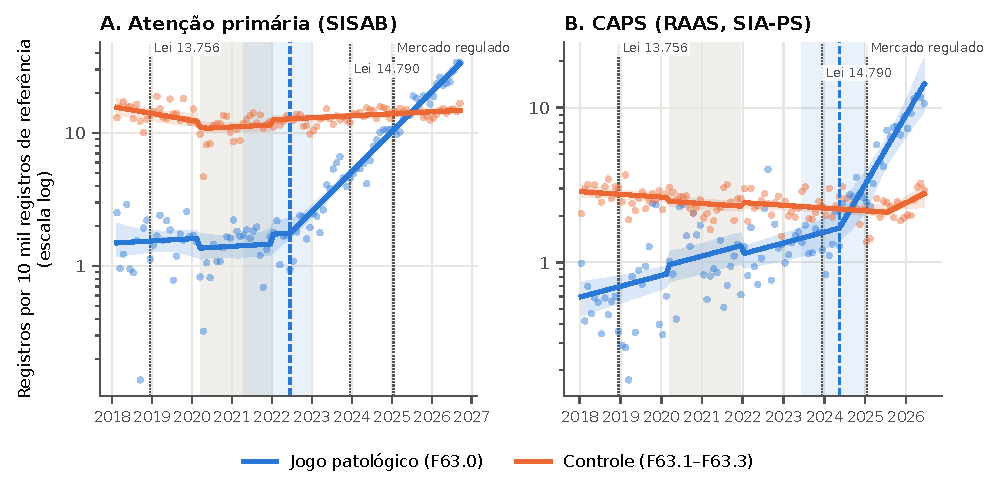
\includegraphics[width=\linewidth]{figuras/figura1}
\caption{Registros de jogo patológico (CID-10 F63.0) e do controle negativo (F63.1--F63.3) por 10 mil registros do grupo de referência, por mês, na atenção primária à saúde (A) e nos Centros de Atenção Psicossocial (B). Brasil, 2018--2026.}
\label{fig:figura1}
\par\smallskip\parbox{\linewidth}{\footnotesize\raggedright Nota: pontos, valores mensais; linhas contínuas, tendência ajustada por regressão segmentada (sem o efeito sazonal), com faixa de IC95\% obtida por \emph{bootstrap}; linha tracejada vertical, mês da mudança de tendência do jogo patológico, e faixa azul vertical, seu IC95\%; faixa cinza, pandemia de COVID-19 (março de 2020 a dezembro de 2021); linhas verticais pontilhadas, Lei nº 13.756/2018, Lei nº 14.790/2023 e início do mercado regulado (janeiro de 2025), apenas como referência temporal. Escala logarítmica. Referência: F32, F33, F41, F43, F10 e F20. Fontes: Sistema de Informação em Saúde para a Atenção Básica (fev/2018 a set/2026); Sistema de Informações Ambulatoriais do SUS, Registro das Ações Ambulatoriais de Saúde (jan/2018 a jun/2026).}
\end{figure}

% Gerado por artigo/analise/para_latex.py a partir de artigo/resultados/numeros.json. Não editar à mão.
\begin{table}[htbp]
\centering
\fontsize{9}{11}\selectfont
\setlength{\tabcolsep}{4pt}
\caption{Mudança de tendência e variação percentual anual das taxas de jogo patológico e do controle negativo e dos registros do grupo de referência na atenção primária à saúde (APS) e nos Centros de Atenção Psicossocial (CAPS). Brasil, 2018--2026.}
\label{tab:tabela2}
\begin{tabular}{>{\raggedright\arraybackslash}p{7.2cm}R{1.4cm}R{2.6cm}R{1.4cm}R{2.6cm}}
\toprule
Indicador & APS & IC95\% (APS) & CAPS & IC95\% (CAPS) \\ \midrule
Jogo patológico: mês da mudança de tendência & jun/2022 & abr/2021--dez/2022 & mai/2024 & jun/2023--jan/2025 \\
Jogo patológico: VPA antes da mudança (\%) & 4 & \textminus{}26; 15 & 18 & 8; 25 \\
Jogo patológico: VPA depois da mudança (\%) & 100 & 91; 110 & 181 & 107; 367 \\
Controle negativo: VPA do último segmento (\%) & 4 & 1; 14 & 35 & \textminus{}1; 61 \\
Registros da referência: VPA do último segmento (\%) & 19 & 18; 20 & 6 & 3; 12 \\
\bottomrule
\end{tabular}
\par\smallskip\parbox{\linewidth}{\raggedright APS: atenção primária à saúde; CAPS: Centros de Atenção Psicossocial; IC95\%: intervalo de 95\% de confiança; VPA: variação percentual anual. Jogo patológico e controle negativo em taxa por 10 mil registros da referência; registros da referência em número absoluto (crescimento da rede). Regressão segmentada (\emph{joinpoint}) binomial negativa, ajustada pelo mês do ano e pela pandemia de COVID-19; IC95\% por \emph{bootstrap} de blocos de seis meses (999 réplicas). Último segmento do controle negativo: desde mai/2020 na APS e desde jul/2025 nos CAPS (IC95\% do mês: fev/2020--jul/2025). Referência: sem mudança de tendência na APS; nos CAPS, queda de jun/2019 a jun/2020 e crescimento desde então. Jogo patológico: F63.0; controle negativo: F63.1--F63.3. Referência: F32, F33, F41, F43, F10 e F20. APS: fev/2018 a set/2026; CAPS: jan/2018 a jun/2026. Fontes: Sistema de Informação em Saúde para a Atenção Básica; Sistema de Informações Ambulatoriais do SUS, Registro das Ações Ambulatoriais de Saúde.}
\end{table}


O resultado se manteve nas análises de sensibilidade: a VPA depois da mudança ficou entre 100\% e 104\% na APS e entre 145\% e 237\% nos CAPS (Figura S1). A exceção foi somar ao desfecho, nos CAPS, os códigos F63 sem especificação, que também cresceram: a VPA caiu para 62\% ao ano. Esses códigos, porém, têm outro perfil: 36\% dos seus registros eram de menores de 18 anos, contra 7\% no jogo patológico.

Em 2025, o jogo patológico se concentrou em adultos de 25 a 44 anos, com 63\% dos registros na APS e 59\% nos CAPS, contra 32\% e 42\% na referência (Figura 2). Na APS, as mulheres foram 47\% dos registros de jogo, contra 22\% em 2022 (Figura S2).

\begin{figure}[!htbp]
\centering
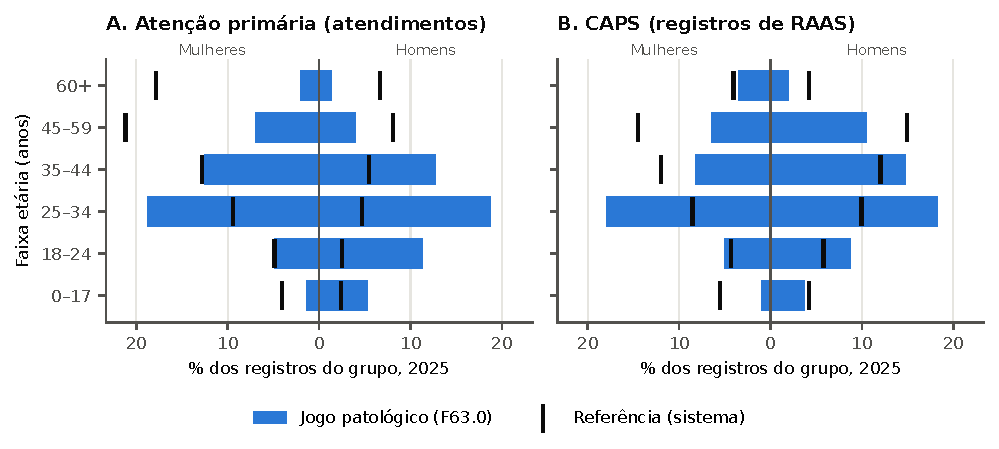
\includegraphics[width=\linewidth]{figuras/figura2}
\caption{Distribuição dos registros de jogo patológico (CID-10 F63.0; barras) e do grupo de referência (traços) por sexo e faixa etária, na atenção primária à saúde (A) e nos Centros de Atenção Psicossocial (B). Brasil, 2025.}
\label{fig:figura2}
\par\smallskip\parbox{\linewidth}{\footnotesize\raggedright Nota: porcentagem dos registros de cada grupo. Registros sem sexo ou idade informados foram excluídos. Referência: F32, F33, F41, F43, F10 e F20. Fontes: Sistema de Informação em Saúde para a Atenção Básica; Sistema de Informações Ambulatoriais do SUS, Registro das Ações Ambulatoriais de Saúde.}
\end{figure}

Na APS, os atendimentos por jogo patológico terminaram menos vezes em alta que os de ansiedade, depressão e uso de álcool e foram encaminhados a serviço especializado com frequência mais de duas vezes maior: 24,2\%, contra 9,9\% a 11,6\% (Tabela 3). O encaminhamento direto ao CAPS foi raro (1,9\%).

% Gerado por artigo/analise/para_latex.py a partir de artigo/resultados/numeros.json. Não editar à mão.
\begin{table}[htbp]
\centering
\fontsize{9}{11}\selectfont
\setlength{\tabcolsep}{4pt}
\caption{Conduta registrada ao fim dos atendimentos na atenção primária à saúde, por diagnóstico. Brasil, janeiro de 2025 a set/2026.}
\label{tab:tabela3}
\begin{tabular}{>{\raggedright\arraybackslash}p{2.5cm}R{1.9cm}R{1.4cm}R{2.0cm}R{2.0cm}R{2.5cm}R{2.4cm}}
\toprule
Diagnóstico & Atendimentos (n) & Alta do episódio (\%) & Retorno para consulta agendada (\%) & Retorno para cuidado continuado (\%) & Encaminhamento para serviço especializado (\%) & Encaminhamento para CAPS (\%) \\ \midrule
Jogo patológico (F63.0) & 8.919 & 37,6 & 35,2 & 31,4 & 24,2 & 1,9 \\
Ansiedade (F41) & 2.387.047 & 48,6 & 27,9 & 28,7 & 9,9 & 0,2 \\
Depressão (F32) & 753.674 & 48,6 & 27,4 & 29,5 & 11,6 & 0,6 \\
Uso de álcool (F10) & 66.420 & 54,3 & 24,4 & 25,4 & 11,3 & 1,8 \\
\bottomrule
\end{tabular}
\par\smallskip\parbox{\linewidth}{\raggedright CAPS: Centro de Atenção Psicossocial. Um atendimento pode ter mais de uma conduta, e as linhas não somam 100\%. O registro não identifica o serviço especializado. Fonte: Sistema de Informação em Saúde para a Atenção Básica.}
\end{table}


\section{Discussão}

\pendente{A ESCREVER: discutir os resultados; o que ainda pode ser feito; jogo e comorbidade com depressão e ansiedade. Limitações a cobrir, vindas da análise: registro não é pessoa, e sem ligação de registros não se separa caso novo de acompanhamento; o controle negativo capta mudanças gerais de codificação, mas não as que favorecem o F63.0 em particular (atenção da mídia, Lei nº 14.790, orientações do Ministério da Saúde), de modo que aumento de demanda e aumento de reconhecimento não se separam; parte da alta nos CAPS pode ser codificação mais específica dentro do F63; antes de 2021, os registros de jogo nos CAPS são poucos e concentrados em poucos serviços; o modelo não tem saltos de nível e algumas séries têm autocorrelação residual; o desenho é ecológico e não estima prevalência nem o efeito de uma lei; o plano de análise não foi registrado antes.}

\section{Conclusão}

\pendente{A ESCREVER}

% ---------------------------------------------------------------------------------------------------------------------
\bibliographystyle{vancouver}
\bibliography{bibliography}

% ---------------------------------------------------------------------------------------------------------------------
\clearpage
\section*{Material Suplementar}
\setcounter{figure}{0}
\renewcommand{\thefigure}{S\arabic{figure}}

\begin{figure}[!htbp]
\centering
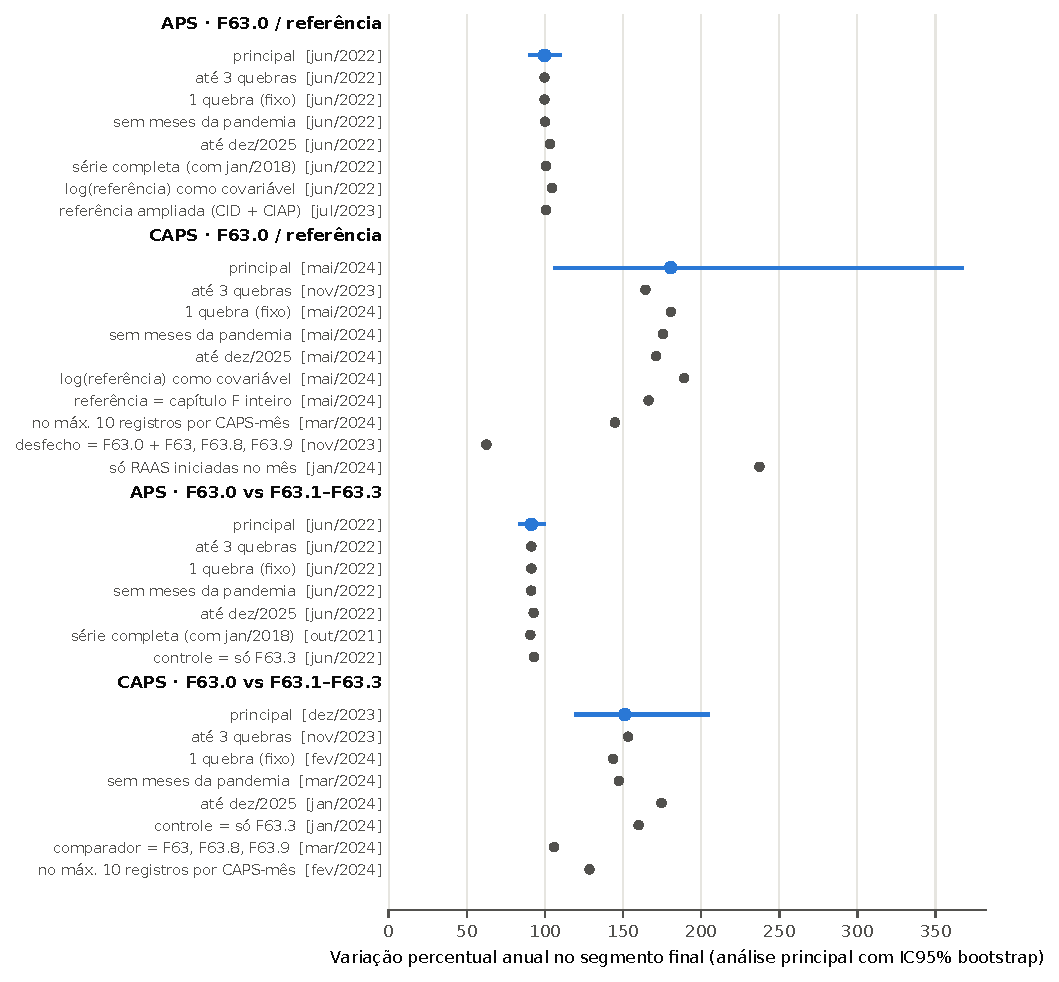
\includegraphics[width=\linewidth]{figuras/figuraS1}
\caption{Variação percentual anual (VPA) da taxa de jogo patológico (CID-10 F63.0) por 10 mil registros do grupo de referência depois da última mudança de tendência, em cada análise de sensibilidade. Entre colchetes, o mês da mudança. Em azul, a análise principal, com IC95\% por \emph{bootstrap}. As duas últimas seções mostram a razão entre os registros de jogo patológico e os do controle negativo (F63.1--F63.3), modelada por regressão binomial. APS, atenção primária à saúde; CAPS, Centros de Atenção Psicossocial.}
\label{fig:figuraS1}
\end{figure}

\begin{figure}[!htbp]
\centering
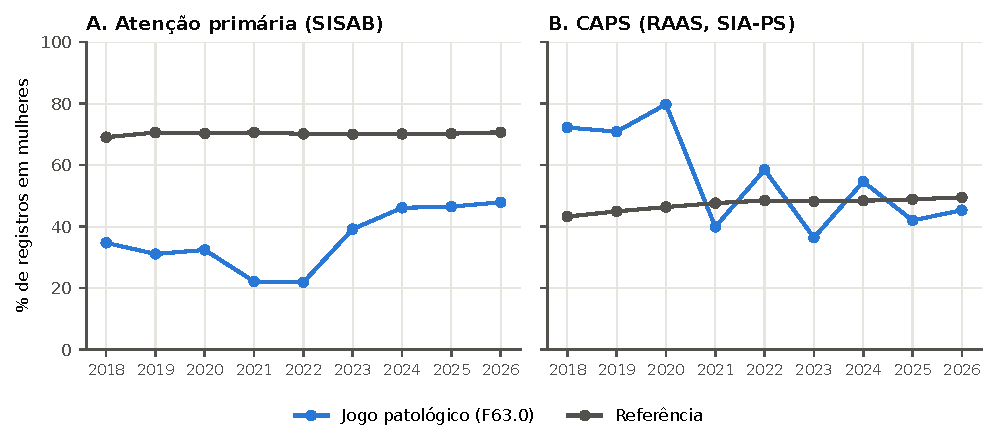
\includegraphics[width=\linewidth]{figuras/figuraS2}
\caption{Porcentagem de registros em mulheres por ano, jogo patológico (CID-10 F63.0) e grupo de referência, na atenção primária à saúde (A) e nos Centros de Atenção Psicossocial (B). Brasil, 2022--2026. Sem intervalos de confiança, porque registros de uma mesma pessoa não são independentes.}
\label{fig:figuraS2}
\end{figure}

\end{document}
